%%%%%%%%%%%%%%%%%%%%%%%%%%%%%%%%%%%%%%%%%
%
% CMPT 432
% Spring 2022
% Lab Five
%
%%%%%%%%%%%%%%%%%%%%%%%%%%%%%%%%%%%%%%%%%

%%%%%%%%%%%%%%%%%%%%%%%%%%%%%%%%%%%%%%%%%
% Short Sectioned Assignment
% LaTeX Template
% Version 1.0 (5/5/12)
%
% This template has been downloaded from: http://www.LaTeXTemplates.com
% Original author: % Frits Wenneker (http://www.howtotex.com)
% License: CC BY-NC-SA 3.0 (http://creativecommons.org/licenses/by-nc-sa/3.0/)
% Modified by Alan G. Labouseur  - alan@labouseur.com
%
%%%%%%%%%%%%%%%%%%%%%%%%%%%%%%%%%%%%%%%%%

%----------------------------------------------------------------------------------------
%	PACKAGES AND OTHER DOCUMENT CONFIGURATIONS
%----------------------------------------------------------------------------------------

\documentclass[letterpaper, 10pt,DIV=13]{scrartcl} 

\usepackage[T1]{fontenc} % Use 8-bit encoding that has 256 glyph
\usepackage[english]{babel} % English language/hyphenation
\usepackage{amsmath,amsfonts,amsthm,xfrac} % Math packages
\usepackage{sectsty} % Allows customizing section commands
\usepackage{graphicx}
\usepackage[lined,linesnumbered,commentsnumbered]{algorithm2e}
\usepackage{listings}
\usepackage{parskip}
\usepackage{lastpage}
\usepackage{tikz}

\allsectionsfont{\normalfont\scshape} % Make all section titles in default font and small caps.

\usepackage{fancyhdr} % Custom headers and footers
\pagestyle{fancyplain} % Makes all pages in the document conform to the custom headers and footers

\fancyhead{} % No page header - if you want one, create it in the same way as the footers below
\fancyfoot[L]{} % Empty left footer
\fancyfoot[C]{} % Empty center footer
\fancyfoot[R]{page \thepage\ of \pageref{LastPage}} % Page numbering for right footer

\renewcommand{\headrulewidth}{0pt} % Remove header underlines
\renewcommand{\footrulewidth}{0pt} % Remove footer underlines
\setlength{\headheight}{13.6pt} % Customize the height of the header

\numberwithin{equation}{section} % Number equations within sections (i.e. 1.1, 1.2, 2.1, 2.2 instead of 1, 2, 3, 4)
\numberwithin{figure}{section} % Number figures within sections (i.e. 1.1, 1.2, 2.1, 2.2 instead of 1, 2, 3, 4)
\numberwithin{table}{section} % Number tables within sections (i.e. 1.1, 1.2, 2.1, 2.2 instead of 1, 2, 3, 4)

\setlength\parindent{0pt} % Removes all indentation from paragraphs.

\binoppenalty=3000
\relpenalty=3000

%----------------------------------------------------------------------------------------
%	TITLE SECTION
%----------------------------------------------------------------------------------------

\newcommand{\horrule}[1]{\rule{\linewidth}{#1}} % Create horizontal rule command with 1 argument of height

\title{	
   \normalfont \normalsize 
   \textsc{CMPT 432 - Spring 2022 - Dr. Labouseur} \\[10pt] % Header stuff.
   \horrule{0.5pt} \\[0.25cm] 	% Top horizontal rule
   \huge Lab Seven  \\     	    % Assignment title
   \horrule{0.5pt} \\[0.25cm] 	% Bottom horizontal rule
}

\author{Shannon Cordoni \\ \normalsize Shannon.Cordoni@Marist.edu}

\date{\normalsize\today} 	% Today's date.

\begin{document}
\maketitle % Print the title

%----------------------------------------------------------------------------------------
%   start PROBLEM ONE
%----------------------------------------------------------------------------------------
\section{Problem One: }

\paragraph{} Describe what is happening in the diagram below.

\begin{figure}[ht]
  \centering
  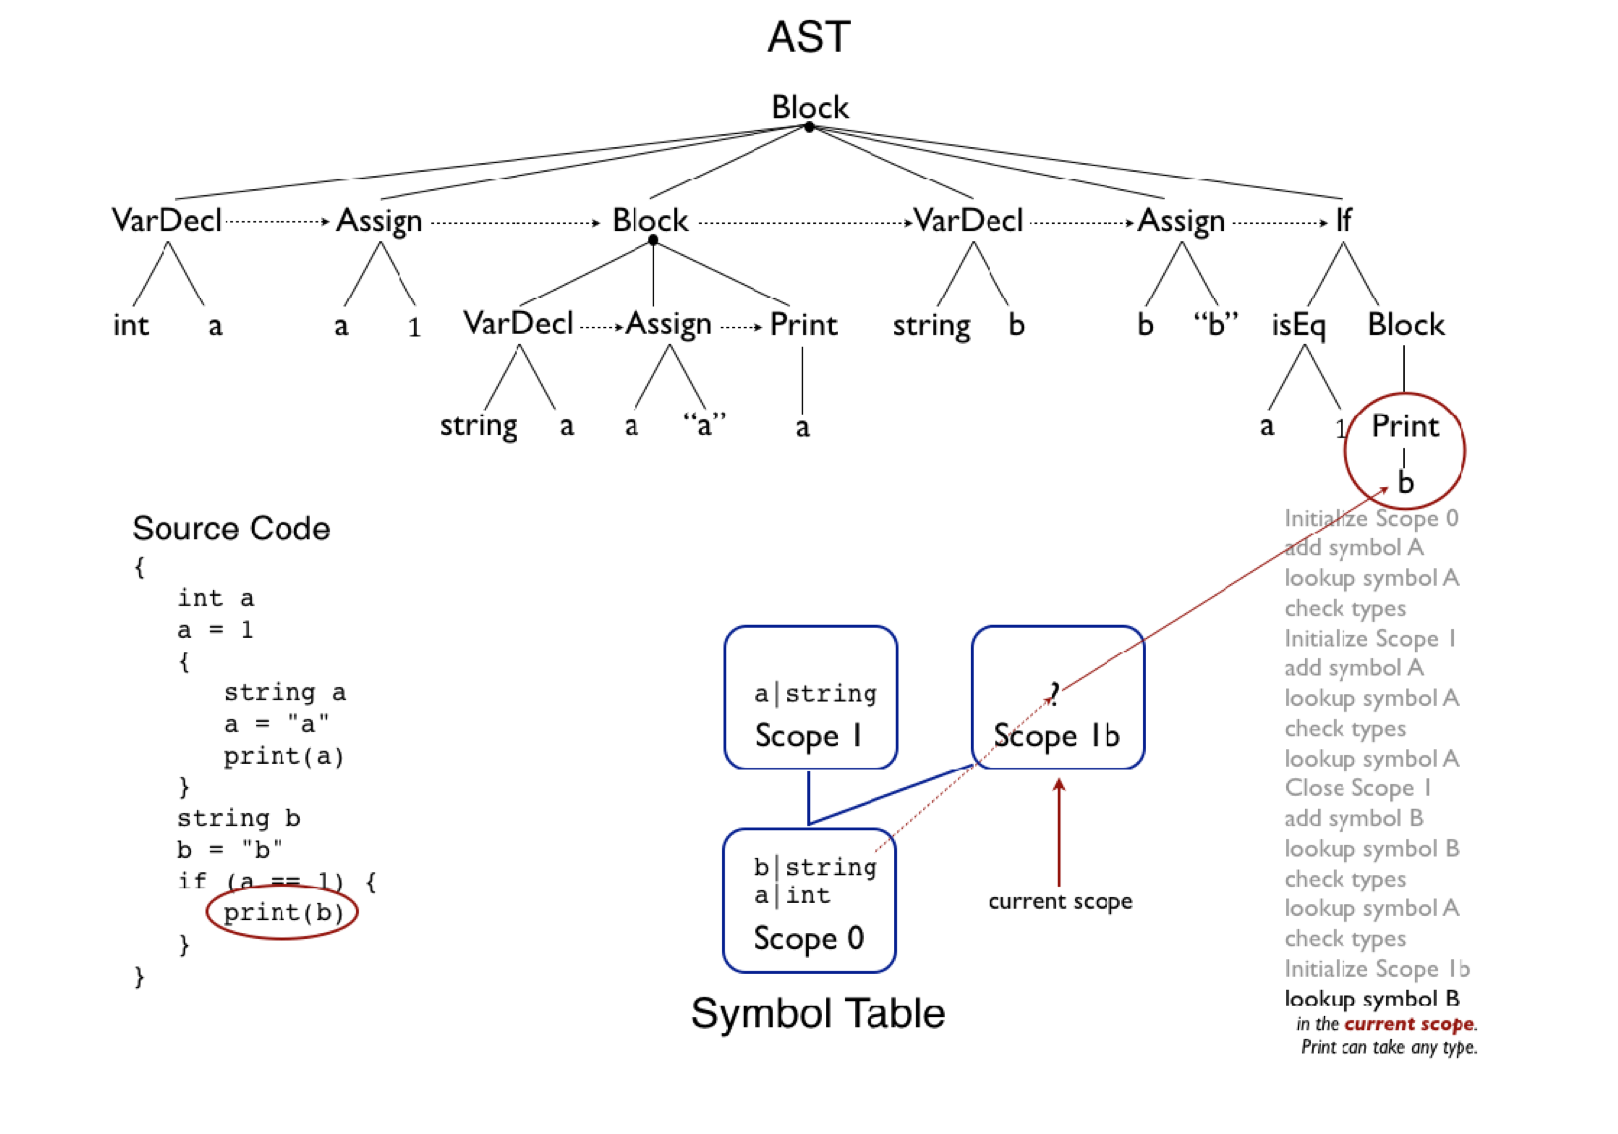
\includegraphics[width=11cm]{IMG_0070.png}
  \label{figure:IMG_0021.png}
\end{figure}

\paragraph{} In the diagram above it appears as if our compiler is walking through the semantic analysis process. Our current red pointers look as if we are processing the line that says "print(b)" and that we are currently looking that the block of code associated with the If Statement. By going through our AST it seems as in the first level or scope of the program we define the variable b as a string. Then once we hit our if statement we define a new block or scope of code to execute should the if statement be true. Since the variable b has been defined in scope 0 or the global scope we are able to access the variable b in scope 1b when calling print. When we hit this block of code we can look up b in our scope 0 hash table and return its value. 


%----------------------------------------------------------------------------------------
%   REFERENCES
%----------------------------------------------------------------------------------------
% The following two commands are all you need in the initial runs of your .Tex file to
% produce the bibliography for the citations in your paper.
\bibliographystyle{abbrv}
\bibliography{lab01} 
% You must have a proper ".bib" file and remember to run:
% latex bibtex latex latex
% to resolve all references.

\pagebreak
\end{document}